\documentclass[11pt,a4paper]{article}

\usepackage{iftex}

\ifpdftex
  \usepackage[utf8]{vietnam}
  \usepackage{tgpagella}
  \usepackage{amsmath, amssymb}
\else
  \usepackage{fontspec}
  \usepackage{unicode-math}
  \setmainfont{texgyrepagella-regular.otf}[
      BoldFont = texgyrepagella-bold.otf,
      ItalicFont = texgyrepagella-italic.otf,
      BoldItalicFont = texgyrepagella-bolditalic.otf
  ]
  \setmathfont{texgyrepagella-math.otf}
  \usepackage{amsmath}
\fi

\usepackage[a4paper, margin=2.5cm]{geometry}
\usepackage{microtype}
\usepackage{titlesec}
\usepackage{enumitem}
\usepackage{multicol}
\usepackage{tikz}
\usetikzlibrary{arrows.meta}

% Căn chỉnh khoảng cách theo chuẩn quy định
\linespread{1.05}
\setlength{\parindent}{0pt}
\setlength{\parskip}{5pt plus 2pt minus 1pt}

% Khoảng cách phương trình toán học
\setlength{\abovedisplayskip}{5pt plus 2pt minus 2pt}
\setlength{\belowdisplayskip}{5pt plus 2pt minus 2pt}
\setlength{\abovedisplayshortskip}{3pt plus 1pt}
\setlength{\belowdisplayshortskip}{3pt plus 1pt}

% Định dạng tiêu đề chương
\titleformat{\section}
  {\large\bfseries}
  {\thesection}{0.5em}{}
\titlespacing*{\section}
  {0pt}{14pt plus 3pt minus 2pt}{6pt plus 1pt minus 1pt}

\titleformat{\subsection}
  {\normalsize\bfseries}
  {\thesubsection}{0.5em}{}
\titlespacing*{\subsection}
  {0pt}{8pt plus 2pt minus 2pt}{2pt plus 1pt minus 1pt}

\titleformat{\subsubsection}
  {\small\bfseries\itshape}
  {\thesubsubsection}{0.5em}{}
\titlespacing*{\subsubsection}
  {0pt}{8pt plus 2pt minus 2pt}{2pt plus 1pt minus 1pt}

\pagestyle{plain}

\begin{document}

\begin{center}
    {\Large\bfseries TỔNG HỢP BÀI TẬP VẬT LÝ ĐIỆN TỬ}\\[0.2cm]
    {\bfseries HỌC PHẦN: PH3330}
\end{center}
\vspace{0.2cm}

%=====================================================================
% CHƯƠNG I
%=====================================================================
\section*{Chương I. Chuyển động của hạt tích điện trong chân không}

\textbf{Bài 1-1.} Tìm biểu thức và xác định độ nhạy của một ống tia điện tử của máy dao động ký có các thông số sau: Hiệu điện thế tăng tốc chùm điện tử là $900\text{ V}$, khoảng cách từ điểm giữa bản lái tia đến màn huỳnh quang bằng $20\text{ cm}$, chiều dài các bản lái tia bằng $2\text{ cm}$, khoảng cách giữa hai bản lái tia bằng $0{,}5\text{ cm}$.

\vspace{0.35cm}

\textbf{Bài 1-2.} Tìm biểu thức và xác định độ nhạy của một ống tia điện tử của máy dao động ký có các thông số sau: Hiệu điện thế tăng tốc chùm điện tử là $900\text{ V}$. Khoảng cách giữa tâm của vùng từ trường làm lệch tia điện tử đến màn huỳnh quang bằng $35\text{ cm}$. Hệ thống lái tia gồm hai cuộn dây Helmholtz hình tròn có bán kính $R = 2{,}5\text{ cm}$ đặt cách nhau một khoảng cách $2z = 5\text{ cm}$. Số vòng dây trên mỗi cuộn là $200$ vòng. Kích thước vùng tác dụng của từ trường là $2R$, trong đó từ trường được xem là đều.

\textit{Chú ý:} Cường độ từ trường trong cuộn Helmholtz được tính bởi công thức:
\begin{equation*}
    H = \frac{i}{2}\frac{WR^2}{(R^2+z^2)^{3/2}}
\end{equation*}
Độ từ thẩm của chân không $\mu_0 = 1{,}26 \cdot 10^{-6}\text{ T}\cdot\text{m/A}$; $i$ là dòng điện trong cuộn dây, $W$ là số vòng dây của cả hai cuộn.

\vspace{0.35cm}

\textbf{Bài 1-3.} Trên đường đi của chùm điện tử người ta đặt một hệ gồm hai lưới có dạng mặt cầu đồng tâm bán kính trung bình là $R = 3\text{ cm}$. Điện thế lưới ngoài là $U_1 = 300\text{ V}$, điện thế lưới trong là $U_2 = 500\text{ V}$ (so với catot phát xạ điện tử). Chứng minh rằng hệ hai lưới này có tính hội tụ đối với chùm điện tử. Tính tiêu cự của hệ (Hình 1.1).

\begin{center}
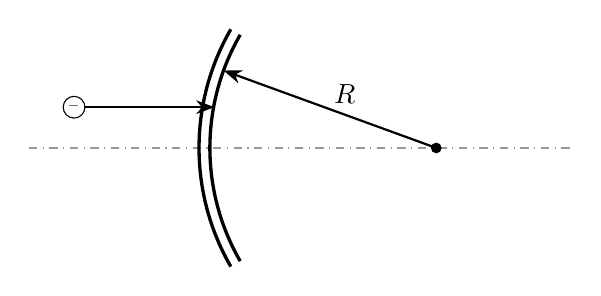
\begin{tikzpicture}[scale=1.15, >=Stealth]
  % Trục quang học
  \draw[dashdotted, thick, gray!80] (-3,0) -- (3,0);
  % Tâm O trên trục quang học
  \filldraw (1.5,0) circle (1.5pt);
  % Hệ hai lưới cầu kép đồng tâm (lồi sang trái hướng về phía electron tới)
  \draw[very thick] ([shift=(150:2.5)] 1.5,0) arc (150:210:2.5);
  \draw[very thick] ([shift=(150:2.62)] 1.5,0) arc (150:210:2.62);
  % Vectơ bán kính R từ tâm O tới mặt lưới
  \draw[->, thick] (1.5,0) -- ++(160:2.5) node[midway, above right=-2pt] {$R$};
  % Hạt điện tử bay song song với trục tới mặt lưới
  \draw (-2.5, 0.45) circle (0.12) node {\tiny $-$};
  \draw[->, thick] (-2.38, 0.45) -- (-0.95, 0.45);
\end{tikzpicture}\\[0.12cm]
\textit{Hình 1.1: Sơ đồ hệ hai lưới cầu cho bài tập (1-3).}
\end{center}

\vspace{0.35cm}

\textbf{Bài 1-4.} Một hệ quang học điện tử gồm một catot phẳng $K$, một lưới tăng tốc $G$ có điện thế $U_G$ bằng $200\text{ V}$, một tấm ngăn (diapham) có điện thế $U_D$ và một anot $A$ được nối với diapham (Hình 1.2). Xác định điện thế $U_D$ (so với catot) để chùm điện tử song song hội tụ lên anot. Cho biết khoảng cách giữa lưới tăng tốc đến diapham là $0{,}5\text{ cm}$, khoảng cách giữa diapham đến anot là $0{,}8\text{ cm}$.

\begin{center}
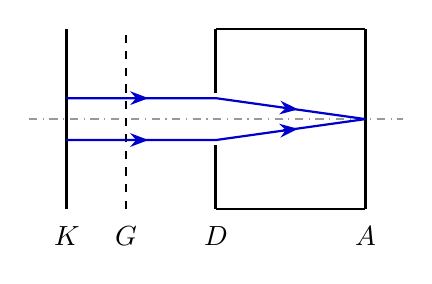
\begin{tikzpicture}[scale=0.95, >=Stealth]
  % Trục quang học
  \draw[dashdotted, thick, gray!80] (-0.5,0) -- (4.5,0);
  % Catot K
  \draw[very thick] (0,-1.2) -- (0,1.2);
  \node[below] at (0,-1.3) {$K$};
  % Lưới tăng tốc G
  \draw[thick, dashed] (0.8,-1.2) -- (0.8,1.2);
  \node[below] at (0.8,-1.3) {$G$};
  % Diapham D (tấm chắn có lỗ)
  \draw[very thick] (2,0.35) -- (2,1.2);
  \draw[very thick] (2,-0.35) -- (2,-1.2);
  \node[below] at (2,-1.3) {$D$};
  % Anot A
  \draw[very thick] (4,-1.2) -- (4,1.2);
  \node[below] at (4,-1.3) {$A$};
  % Khung nối D với A
  \draw[thick] (2,1.2) -- (4,1.2);
  \draw[thick] (2,-1.2) -- (4,-1.2);
  % Quỹ đạo chùm điện tử
  \draw[thick, blue!80!black] (0,0.28) -- (2,0.28) -- (4,0);
  \draw[thick, blue!80!black] (0,-0.28) -- (2,-0.28) -- (4,0);
  % Mũi tên hướng đi
  \draw[->, thick, blue!80!black] (0.9,0.28) -- (1.1,0.28);
  \draw[->, thick, blue!80!black] (0.9,-0.28) -- (1.1,-0.28);
  \draw[->, thick, blue!80!black] (2.9,0.15) -- (3.1,0.13);
  \draw[->, thick, blue!80!black] (2.9,-0.15) -- (3.1,-0.13);
\end{tikzpicture}\\[0.12cm]
\textit{Hình 1.2: Sơ đồ hệ quang học điện tử cho bài tập (1-4).}
\end{center}

\vspace{0.35cm}

\textbf{Bài 1-5.} Xét một hệ quang học điện tử gồm một catot $K$, hai diapham $D_1, D_2$ và một anot $A$ (Hình 1.3). Khoảng cách giữa các điện cực đó bằng nhau và bằng $1\text{ cm}$. Điện thế của diapham thứ nhất $D_1$ bằng điện thế anot $A$ và bằng $U_1 = 100\text{ V}$ (so với điện thế catot $K$). Xác định điện thế của diapham thứ hai $D_2$ để cho chùm điện tử song song đi qua hệ hội tụ ở anot $A$.

\begin{center}
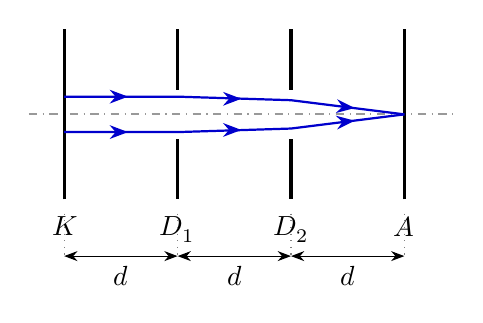
\begin{tikzpicture}[scale=0.9, >=Stealth]
  % Trục quang học
  \draw[dashdotted, thick, gray!80] (-0.5,0) -- (5.5,0);
  % Catot K
  \draw[very thick] (0,-1.2) -- (0,1.2);
  \node[below] at (0,-1.3) {$K$};
  % Diapham D1
  \draw[very thick] (1.6,0.35) -- (1.6,1.2);
  \draw[very thick] (1.6,-0.35) -- (1.6,-1.2);
  \node[below] at (1.6,-1.3) {$D_1$};
  % Diapham D2
  \draw[very thick] (3.2,0.35) -- (3.2,1.2);
  \draw[very thick] (3.2,-0.35) -- (3.2,-1.2);
  \node[below] at (3.2,-1.3) {$D_2$};
  % Anot A
  \draw[very thick] (4.8,-1.2) -- (4.8,1.2);
  \node[below] at (4.8,-1.3) {$A$};
  % Kích thước khoảng cách d
  \draw[<->, thin] (0,-2.0) -- (1.6,-2.0) node[midway, below] {$d$};
  \draw[<->, thin] (1.6,-2.0) -- (3.2,-2.0) node[midway, below] {$d$};
  \draw[<->, thin] (3.2,-2.0) -- (4.8,-2.0) node[midway, below] {$d$};
  % Đường gióng từ điện cực xuống thước đo
  \draw[dotted, gray] (0,-1.4) -- (0,-2.0);
  \draw[dotted, gray] (1.6,-1.4) -- (1.6,-2.0);
  \draw[dotted, gray] (3.2,-1.4) -- (3.2,-2.0);
  \draw[dotted, gray] (4.8,-1.4) -- (4.8,-2.0);
  % Quỹ đạo chùm điện tử
  \draw[thick, blue!80!black] (0,0.25) -- (1.6,0.25) -- (3.2,0.2) -- (4.8,0);
  \draw[thick, blue!80!black] (0,-0.25) -- (1.6,-0.25) -- (3.2,-0.2) -- (4.8,0);
  \draw[->, thick, blue!80!black] (0.8,0.25) -- (0.9,0.25);
  \draw[->, thick, blue!80!black] (0.8,-0.25) -- (0.9,-0.25);
  \draw[->, thick, blue!80!black] (2.4,0.22) -- (2.5,0.22);
  \draw[->, thick, blue!80!black] (2.4,-0.22) -- (2.5,-0.22);
  \draw[->, thick, blue!80!black] (4.0,0.1) -- (4.1,0.09);
  \draw[->, thick, blue!80!black] (4.0,-0.1) -- (4.1,-0.09);
\end{tikzpicture}\\[0.12cm]
\textit{Hình 1.3: Sơ đồ hệ quang học điện tử hai diapham cho bài tập (1-5).}
\end{center}

\newpage

%=====================================================================
% CHƯƠNG II
%=====================================================================
\section*{Chương II. Một số vấn đề vật lý lượng tử}

\textbf{Bài 2-1.} Một mặt bằng kali ở cách ngọn đèn $100\text{ W}$ là $75\text{ cm}$. Giả thiết năng lượng bức xạ của đèn trong đơn vị thời gian chỉ bằng $5\%$ công suất định mức. Nếu coi mỗi nguyên tử kali có dạng một đĩa dẹt đường kính $1\text{ \AA}$, hãy xác định thời gian cần thiết để mỗi nguyên tử đó hấp thụ một năng lượng bằng công thoát của nó $\varphi_K \cong 2\text{ eV}$, theo mẫu sóng ánh sáng. Rút ra nhận xét.

\vspace{0.35cm}

\textbf{Bài 2-2.} Người ta chiếu kali bằng tia cực tím bước sóng $2500\text{ \AA}$. Biết công thoát của kali là $2{,}2\text{ eV}$, tính động năng cực đại của các electron phát ra. Nếu cường độ bức xạ tới là $2\text{ W/m}^2$, tính số điện tử do một đơn vị diện tích phát ra trong một đơn vị thời gian.

\vspace{0.35cm}

\textbf{Bài 2-3.} Một photon X năng lượng $0{,}3\text{ MeV}$ va chạm trực diện với một electron lúc đầu ở trạng thái nghỉ. Tính vận tốc lùi của electron bằng cách áp dụng các nguyên lý bảo toàn năng lượng và xung lượng. Kiểm tra lại kết quả bằng công thức Compton.

\vspace{0.35cm}

\textbf{Bài 2-4.} Tính hiệu điện thế gia tốc cần thiết để bước sóng kết hợp với một electron (sóng De Broglie) có bước sóng $1\text{ \AA}$ (vào cỡ khoảng cách giữa các nguyên tử trong tinh thể).

\vspace{0.35cm}

\textbf{Bài 2-5.} Chứng tỏ rằng khi một hạt có năng lượng rất lớn so với năng lượng nghỉ của nó thì hạt sẽ có bước sóng kết hợp gần đúng bằng bước sóng của photon có cùng năng lượng.

\vspace{0.35cm}

\textbf{Bài 2-6.} Tính vận tốc pha và vận tốc nhóm của một sóng De Broglie có bước sóng $\lambda = h/p = h/mv$.

\vspace{0.35cm}

\textbf{Bài 2-7.} Một chùm hẹp electron năng lượng $60\text{ keV}$ đi xuyên qua một màng đa tinh thể bạc (Ag) có khoảng cách giữa mặt mạng là $d = 4{,}08\text{ \AA}$. Xác định bán kính ảnh nhiễu xạ bậc nhất trên màn hình đặt ở sau màng bạc $40\text{ cm}$.

\vspace{0.35cm}

\textbf{Bài 2-8.} Ta giả thiết $h = 6{,}625 \cdot 10^{-3}\text{ J}\cdot\text{s}$ thay cho $6{,}625 \cdot 10^{-34}\text{ J}\cdot\text{s}$. Người ta ném các viên bi khối lượng $66{,}25\text{ g}$ với vận tốc $5\text{ m/s}$ xuyên qua hai cửa sổ hẹp, song song và cách nhau $0{,}6\text{ m}$. Mỗi lần ném, viên bi lọt qua cửa sổ nào là hoàn toàn ngẫu nhiên. Tính khoảng cách vân của ảnh giao thoa trên tường cách phía sau cửa sổ $12\text{ m}$.

\vspace{0.35cm}

\textbf{Bài 2-9.} Giả sử ta có thể đo được xung lượng của một hạt đến phần nghìn. Xác định độ bất định cực tiểu về vị trí của hạt:
\begin{enumerate}[label=\alph*)]
  \item Nếu hạt có khối lượng $5\text{ mg}$ và vận tốc $2\text{ m/s}$.
  \item Nếu hạt là điện tử có vận tốc $1{,}8 \cdot 10^8\text{ m/s}$.
\end{enumerate}

\vspace{0.35cm}

\textbf{Bài 2-10.} Độ rộng của một vạch quang phổ bước sóng $4000\text{ \AA}$ bằng $10^{-4}\text{ \AA}$. Tính thời gian trung bình để hệ nguyên tử ở trạng thái năng lượng đó.

\vspace{0.35cm}

\textbf{Bài 2-11.} Giả sử độ bất định về xung lượng của một hạt đúng bằng xung lượng của nó. Tìm hệ thức giữa độ bất định cực tiểu về vị trí hạt và bước sóng De Broglie của nó.

\vspace{0.35cm}

\textbf{Bài 2-12.} Giả thiết năng lượng của một hạt đang chuyển động theo đường thẳng là $E = \frac{1}{2}mv^2$, chứng minh rằng $\Delta E \cdot \Delta t \ge h/2\pi$, trong đó $\Delta t = \Delta x / v$.

\vspace{0.35cm}

\textbf{Bài 2-13.} Một hạt khối lượng $m$ bị bắt buộc phải ở trên đoạn thẳng $L$. Dựa vào nguyên lý bất định hãy xác định năng lượng cực tiểu mà hạt có thể có. Nếu trong hạt nhân, có đường kính $10^{-14}\text{ m}$, có mặt một điện tử thì động năng cực tiểu của nó bằng bao nhiêu?

\vspace{0.35cm}

\textbf{Bài 2-14.} Tìm hàm riêng và trị riêng của toán tử $\hat{L} = i \frac{d}{dx}$. Qua đó chứng minh rằng hình chiếu xung lượng của hạt tự do là đại lượng không bị lượng tử hoá.

\vspace{0.35cm}

\textbf{Bài 2-15.} Một vi khuẩn rất nhỏ (tiny bacterium) có khối lượng $10^{-14}\text{ kg}$ bị nhốt giữa hai vách cứng cách nhau $0{,}1\text{ mm}$. Xác định vận tốc nhỏ nhất của nó. Nếu vận tốc của nó khoảng $1\text{ mm}$ trong $100\text{ s}$, hãy xác định số lượng tử ứng với trạng thái đó của nó.

\vspace{0.35cm}

\textbf{Bài 2-16.} Một điện tử có động năng $50\text{ eV}$ đến gần một hàng rào thế hình chữ nhật có chiều cao $70\text{ eV}$ và bề dày là:
\begin{enumerate}[label=\alph*)]
  \item $L = 1{,}0\text{ nm}$
  \item $L = 0{,}1\text{ nm}$
\end{enumerate}
Hãy tính xác suất điện tử đi qua theo hiệu ứng đường ngầm.

\vspace{0.35cm}

\textbf{Bài 2-17.} Chứng minh rằng biên độ $A$ của các hàm sóng mô tả các trạng thái của hạt trong một hố thế năng có vách cao vô cực là $A = \sqrt{2/L}$, trong đó $L$ là bề rộng của hố thế.

\vspace{0.35cm}

\textbf{Bài 2-18.} Xét một điện tử nhốt trong một hố thế có vách vô cực, bề rộng $L = 10^{-10}\text{ m}$.
\begin{enumerate}[label=\alph*)]
  \item Tính ba mức năng lượng thấp nhất của điện tử.
  \item Nếu một photon được phát ra khi điện tử chuyển từ mức có $n = 2$ xuống mức có $n = 1$ thì bước sóng của photon bằng bao nhiêu?
\end{enumerate}

\newpage

%=====================================================================
% CHƯƠNG III
%=====================================================================
\section*{Chương III. Cấu trúc nguyên tử và phổ nguyên tử}

\textbf{Bài 3-1.} Tính bước sóng ngắn nhất và bước sóng dài nhất (bằng $\text{\AA}$) đối với dãy Liman của nguyên tử hydro.

\vspace{0.35cm}

\textbf{Bài 3-2.} Tính năng lượng ion hoá của nguyên tử hydro biết rằng bước sóng ngắn nhất của dãy Balmer là $3650\text{ \AA}$.

\vspace{0.35cm}

\textbf{Bài 3-3.} Trong một ống phóng điện các nguyên tử hydro chịu tác dụng của một dòng điện tử năng lượng $12{,}2\text{ eV}$. Tìm bước sóng của các vạch do hydro phát ra.

\vspace{0.35cm}

\textbf{Bài 3-4.} Tính mômen từ của một điện tử chuyển động xung quanh một proton trên một quỹ đạo tròn bán kính $r$ (theo vật lý cổ điển).

\vspace{0.35cm}

\textbf{Bài 3-5.} Áp dụng kết quả của cơ học lượng tử tính các giá trị có thể có của mômen từ đối với mức $n = 3$. Biết công thức liên hệ giữa mômen động lượng và mômen từ:
\begin{equation*}
    \vec{\mu}_l = -\frac{e}{2m}\vec{M}_l
\end{equation*}
với $\vec{\mu}_l$ là vectơ mômen từ quỹ đạo.

\vspace{0.35cm}

\textbf{Bài 3-6.} Biểu diễn các cách định hướng có thể có của mômen động lượng $\vec{M}_l$ với $l = 0, 1, 2$ và $3$ bằng hình vẽ.

\vspace{0.35cm}

\textbf{Bài 3-7.} Trong vật lý thiên văn người ta dùng vạch phổ có bước sóng $21\text{ cm}$ để thăm dò vũ trụ. Vạch này được tạo bởi photon phát ra từ nguyên tử hydro của thiên hà khi hướng của spin của điện tử chuyển từ trạng thái song song sang trạng thái phản song song với spin của proton. Tìm giá trị từ trường tác dụng lên điện tử. Biết rằng công thức liên hệ giữa mômen động lượng spin và mômen từ spin là:
\begin{equation*}
    \vec{\mu}_s = -\frac{e}{m}\vec{M}_s
\end{equation*}
Năng lượng tương tác giữa mômen từ $\vec{\mu}$ và từ trường có vectơ cảm ứng từ $\vec{B}$ là:
\begin{equation*}
    E_B = -\vec{\mu}\vec{B}
\end{equation*}

\vspace{0.35cm}

\textbf{Bài 3-8.} Chứng minh rằng các nguyên tử gồm các lớp điền đầy hoàn toàn sẽ có một trạng thái cơ bản $^1S_0$.

\vspace{0.35cm}

\textbf{Bài 3-9.} Thiết lập cấu hình (cấu trúc) điện tử của 5 khí trơ đầu tiên trong bảng tuần hoàn.

\newpage

%=====================================================================
% CHƯƠNG IV
%=====================================================================
\section*{Chương IV. Một số vấn đề vật lý bán dẫn}

\textbf{Bài 4-1.} Nồng độ hạt dẫn trong bán dẫn riêng thay đổi như thế nào khi nhiệt độ chất bán dẫn thay đổi từ $200\text{ K}$ đến $300\text{ K}$ và bề rộng vùng cấm giả thiết thay đổi theo quy luật $\Delta E_g(T) = (0{,}785 - \alpha T)\text{ eV}$.

\vspace{0.35cm}

\textbf{Bài 4-2.} Bằng thực nghiệm người ta xác định được nồng độ điện tử ở $400\text{ K}$ là $1{,}3 \cdot 10^{16}\text{ cm}^{-3}$ và ở $350\text{ K}$ là $6{,}2 \cdot 10^{16}\text{ cm}^{-3}$. Bán dẫn là tinh khiết, hãy tính bề rộng vùng cấm ở nhiệt độ không tuyệt đối nếu biết rằng $\Delta E_g$ phụ thuộc vào nhiệt độ theo công thức $\Delta E_g(T) = \Delta E_g(0) - \alpha T$.

\vspace{0.35cm}

\textbf{Bài 4-3.} Tính nồng độ điện tử, lỗ trống, vị trí mức Fermi (so với đỉnh vùng hóa trị) của silic chứa $1{,}1 \cdot 10^{16}\text{ nguyên tử B trên } 1\text{ cm}^3$ ở nhiệt độ $300\text{ K}$. Các đại lượng trên sẽ thay đổi như thế nào khi pha thêm vào mẫu các nguyên tử photpho với nồng độ $9 \cdot 10^{15}\text{ nguyên tử P trên } 1\text{ cm}^3$.

Cho biết nồng độ hạt dẫn riêng trong silic ở $300\text{ K}$ là $n_i = 1{,}45 \cdot 10^{10}\text{ cm}^{-3}$, $\Delta E_g = 1{,}12\text{ eV}$, $N_c = 2{,}8 \cdot 10^{19}\text{ cm}^{-3}$, $N_v = 1 \cdot 10^{19}\text{ cm}^{-3}$.

\vspace{0.35cm}

\textbf{Bài 4-4.} Hãy chứng minh công thức nồng độ điện tử trong bán dẫn suy biến loại $n$:
\begin{equation*}
    n_0 = \frac{8\pi}{3}\left(\frac{2m}{h^2}\right)^{3/2}(E_f - E_c)^{3/2}
\end{equation*}
xuất phát từ nguyên lý bất định Heisenberg:
\begin{equation*}
    \Delta x \cdot \Delta p_x = h, \quad \Delta y \cdot \Delta p_y = h, \quad \Delta z \cdot \Delta p_z = h
\end{equation*}

\vspace{0.35cm}

\textbf{Bài 4-5.} Giả sử bán dẫn Si loại $n^+$ với $N_d = 10^{17}\text{ cm}^{-3}$ tiếp xúc với Si loại $n$ với $N_d = 10^{14}\text{ cm}^{-3}$. Hãy tính mức Fermi (so với đáy vùng dẫn) trong từng vật liệu nếu giả thiết bán dẫn không suy biến.

Khi cân bằng nhiệt động mức Fermi trong hai vật liệu là bằng nhau, hãy vẽ định tính sơ đồ vùng năng lượng.

Giải bài toán khi mẫu thứ hai là loại $p$ với $N_a = 10^{14}\text{ cm}^{-3}$. Cho biết $N_c = 2{,}8 \cdot 10^{19}\text{ cm}^{-3}$, $N_v = 1 \cdot 10^{19}\text{ cm}^{-3}$.

\vspace{0.35cm}

\textbf{Bài 4-6.} Tính độ dẫn của silic tinh khiết ở $300\text{ K}$. Biết $n_i = 1{,}45 \cdot 10^{10}\text{ cm}^{-3}$. Độ linh động của điện tử $\mu_n = 1450\text{ cm}^2/\text{V}\cdot\text{s}$; độ linh động của lỗ trống $\mu_p = 450\text{ cm}^2/\text{V}\cdot\text{s}$.

Giải bài toán khi silic được pha thêm một nồng độ asen với nồng độ $1 \cdot 10^{14}\text{ nguyên tử trên } 1\text{ cm}^3$.

Giải bài toán khi silic được pha thêm tiếp tục một nồng độ nhôm là $1 \cdot 10^{17}\text{ nguyên tử trên } 1\text{ cm}^3$.

\vspace{0.35cm}

\textbf{Bài 4-7.} Tính hiệu công thoát điện tử giữa hai mẫu silic, mẫu thứ nhất pha tạp loại $n$ với $N_d = 1 \cdot 10^{15}\text{ cm}^{-3}$, mẫu thứ hai pha tạp loại $p$ với $N_a = 1 \cdot 10^{15}\text{ cm}^{-3}$. Cho biết $\Delta E_g = 1{,}12\text{ eV}$, nhiệt độ $300\text{ K}$ với $kT = 0{,}026\text{ eV}$, $N_c = 2{,}8 \cdot 10^{19}\text{ cm}^{-3}$, $N_v = 1 \cdot 10^{19}\text{ cm}^{-3}$.

Nếu hai mẫu này tiếp xúc với nhau, trong điều kiện cân bằng tính hàng rào thế năng đối với điện tử giữa hai mẫu.

\vspace{0.35cm}

\textbf{Bài 4-8.} Tính bề dày và điện dung lớp chuyển tiếp $p - n$, biết:
\begin{itemize}[itemsep=1pt, topsep=2pt, leftmargin=1.8em]
  \item Thiên áp ngược $U_{\text{ng}} = 20\text{ V}$.
  \item Hằng số điện môi tương đối $\varepsilon = 16$.
  \item Nồng độ pha tạp bên phần $p$ là $N_a = 4 \cdot 10^{21}\text{ m}^{-3}$.
  \item Nồng độ pha tạp bên phần $n$ là $N_d = 2 \cdot 10^{21}\text{ m}^{-3}$.
  \item Diện tích lớp chuyển tiếp $S = 10^{-6}\text{ m}^2$.
  \item Hàng rào thế năng khi thiên áp bằng không là $eU_k = 0{,}5\text{ eV}$.
\end{itemize}

\vspace{0.35cm}

\textbf{Bài 4-9.} Cho một chuyển tiếp $p - n$ trên tinh thể Ge với $\varepsilon = 16$, $N_a = 5 \cdot 10^{22}\text{ m}^{-3}$, $N_d = 1 \cdot 10^{22}\text{ m}^{-3}$. Hỏi với thiên áp ngược bằng bao nhiêu thì xảy ra hiệu ứng đường ngầm qua lớp chuyển tiếp. Biết rằng điện trường tới hạn để xảy ra hiệu ứng đường ngầm là $\mathcal{E}_c = 10^7\text{ V/cm}$. Bỏ qua giá trị hiệu thế tiếp xúc $U_k$.

\vspace{0.35cm}

\textbf{Bài 4-10.} Giả sử grad điện thế trong mẫu silic tinh khiết là $400\text{ V/cm}$, độ linh động của điện tử và lỗ trống tương ứng là $0{,}12\text{ m}^2/\text{V}\cdot\text{s}$ và $0{,}025\text{ m}^2/\text{V}\cdot\text{s}$. Hãy xác định:
\begin{enumerate}[label=\alph*)]
  \item Tốc độ cuốn của điện tử và lỗ trống.
  \item Điện trở suất của silic, giả sử nồng độ hạt dẫn riêng là $2{,}5 \cdot 10^{16}\text{ m}^{-3}$.
  \item Dòng cuốn toàn phần, nếu tiết diện ngang của mẫu là $0{,}03 \cdot 10^{-4}\text{ m}^2$.
\end{enumerate}

\newpage

%=====================================================================
% CHƯƠNG V
%=====================================================================
\section*{Chương V. Xử lý tín hiệu quang -- Quang điện tử}

\textbf{Bài 5-1.} Chứng minh công thức tính khẩu độ số ($NA$ -- Numerical Aperture):
\begin{equation*}
    NA = (n_1^2 - n_2^2)^{1/2} \simeq n_1(2\Delta)^{1/2}
\end{equation*}

\vspace{0.35cm}

\textbf{Bài 5-2.} Từ điều kiện các mode dẫn truyền trong sợi quang giật cấp đa mode, bỏ qua sự dịch chuyển pha do phản xạ ở mặt phân cách lõi -- vỏ, đánh giá số lượng các mode đó cho $d = 10\lambda_0$, $n_1 = 1{,}5$, độ chênh chiết suất $\Delta = 0{,}02$.

\vspace{0.35cm}

\textbf{Bài 5-3.} Cho sợi quang giật cấp đa mode có độ chênh chiết suất $\Delta = 0{,}01$, chiết suất của lõi $1{,}5$, bước sóng ánh sáng $\lambda = 1{,}5\text{ }\mu\text{m}$. Tính độ giãn xung sáng, đánh giá bề rộng dải thông và khẩu độ số (tính góc $\theta_{z\max}$) cho khoảng cách $10\text{ km}$.

\vspace{0.35cm}

\textbf{Bài 5-4.} Cho một bán dẫn vùng cấm thẳng tinh khiết có bề rộng vùng cấm $\Delta E_g = 1{,}5\text{ eV}$, giả sử khối lượng hiệu dụng của điện tử và lỗ trống là đẳng hướng, bằng nhau và bằng $\frac{m_0}{10} = 9{,}1 \cdot 10^{-32}\text{ kg}$.
\begin{enumerate}[label=\alph*)]
  \item Tính bước sóng ngưỡng hấp thụ.
  \item Người ta thấy rằng khi cường độ ánh sáng kích thích quá lớn, bán dẫn trở nên trong suốt với ánh sáng có bước sóng ngưỡng trên đây. Hãy giải thích hiện tượng này.
  \item Nếu mật độ trạng thái trong vùng dẫn và vùng hóa trị được tính theo công thức:
  \begin{equation*}
      g(E) = 2\pi\left(\frac{2m^*}{h^2}\right)^{3/2}\sqrt{E - E_c}
  \end{equation*}
  và nếu cho nồng độ điện tử và nồng độ lỗ trống do quang phát sinh là $10^{18}\text{ cm}^{-3}$, hãy tính bước sóng ngưỡng trong trường hợp này.
\end{enumerate}

\vspace{0.35cm}

\textbf{Bài 5-5.} Một mẫu bán dẫn đơn tinh thể silic có bề dày $0{,}25\text{ }\mu\text{m}$ được chiếu sáng bằng ánh sáng đơn sắc có $h\nu = 3\text{ eV}$ với công suất $10\text{ mW}$. Tìm năng lượng tổng cộng mà mẫu hấp thụ trong $1$ giây, năng lượng nhiệt truyền cho mạng tinh thể trong $1\text{ s}$ và số photon sinh ra do tái hợp bức xạ riêng (vùng -- vùng) cho hệ số hấp thụ ở bước sóng đang xét là $4 \cdot 10^4\text{ cm}^{-1}$, $\Delta E_g = 1{,}12\text{ eV}$.

\vspace{0.35cm}

\textbf{Bài 5-6.} Một mẫu GaAs được chiếu sáng bởi ánh sáng có bước sóng $\lambda = 0{,}6\text{ }\mu\text{m}$. Công suất tia tới là $15\text{ mW}$. Nếu $1/3$ công suất đó bị phản xạ trở lại và $1/3$ thoát ra từ mặt sau của mẫu thì bề dày của mẫu bằng bao nhiêu? Tìm năng lượng nhiệt được truyền cho mạng tinh thể trong một giây. Biết hệ số hấp thụ $\alpha(0{,}6\text{ }\mu\text{m}) = 5 \cdot 10^4\text{ cm}^{-1}$, $\Delta E_g = 1{,}42\text{ eV}$.

\vspace{0.35cm}

\textbf{Bài 5-7.} \textit{(Giảm tải theo đề cương)} Một quang dẫn có kích thước $L = 6\text{ mm}$, $W = 2\text{ mm}$, $D = 1\text{ mm}$ được chiếu bởi bức xạ đồng đều. Do hấp thụ ánh sáng dòng điện tăng lên $2{,}83\text{ mA}$. Điện áp đặt lên $2$ cực là $10\text{ V}$. Khi ngắt nguồn sáng đột ngột dòng điện giảm với vận tốc ban đầu là $23{,}6\text{ A/s}$. Cho biết $\mu_n = 3600\text{ cm}^2/\text{V}\cdot\text{s}$, $\mu_p = 1700\text{ cm}^2/\text{V}\cdot\text{s}$.\\
Tìm:
\begin{enumerate}[label=\alph*)]
  \item Số các điện tử lỗ trống phát sinh trong chế độ dừng;
  \item Thời gian sống của hạt dẫn không cơ bản;
  \item Nồng độ hạt dẫn dư tồn tại sau khi ngắt nguồn sáng $1\text{ ms}$.
\end{enumerate}

\newpage

%=====================================================================
% ĐÁP SỐ TỔNG HỢP
%=====================================================================
\begingroup
\setlength{\multicolsep}{4pt}
\titlespacing*{\section}{0pt}{2pt}{4pt}
\titlespacing*{\subsection}{0pt}{5pt plus 1pt minus 1pt}{1pt}
\setlength{\parskip}{2pt}

\section*{ĐÁP SỐ CÁC CHƯƠNG}

\begin{multicols}{2}
\subsection*{Chương I}
\begin{itemize}[itemsep=0.5pt, topsep=1pt, parsep=0pt, leftmargin=1.8em]
  \item \textbf{(1-1)} $S = 4{,}5 \cdot 10^{-4}\text{ m/V}$
  \item \textbf{(1-2)} $S = 0{,}618\text{ m/A}$
  \item \textbf{(1-3)} $f = 13{,}25 \cdot 10^{-2}\text{ m}$
  \item \textbf{(1-4)} $U_D = 57\text{ V}$
  \item \textbf{(1-5)} Hai nghiệm: $432\text{ V}$ và $28\text{ V}$
\end{itemize}

\columnbreak

\subsection*{Chương III}
\begin{itemize}[itemsep=0.5pt, topsep=1pt, parsep=0pt, leftmargin=1.8em]
  \item \textbf{(3-1)} $\lambda_{\max} = 1215\text{ \AA}$, $\lambda_{\min} = 912\text{ \AA}$
  \item \textbf{(3-2)} $E_i = 13{,}6\text{ eV}$
  \item \textbf{(3-3)} Có 3 loại photon: $\lambda_1 = 6563\text{ \AA}$, $\lambda_2 = 1215\text{ \AA}$, $\lambda_3 = 1026\text{ \AA}$
\end{itemize}
\end{multicols}

\subsection*{Chương II}
\begin{multicols}{2}
\begin{itemize}[itemsep=0.5pt, topsep=1pt, parsep=0pt, leftmargin=1.8em]
  \item \textbf{(2-1)} $t = 57{,}6\text{ s}$
  \item \textbf{(2-2)} $T_{\max} = 2{,}75\text{ eV}$; $J_e = 2{,}52 \cdot 10^{18}\text{ e}/(\text{m}^2\cdot\text{s})$
  \item \textbf{(2-3)} $v = 0{,}65c$
  \item \textbf{(2-4)} $U = 151\text{ V}$
  \item \textbf{(2-5)} $\lambda_\gamma = \frac{hc}{E} = \lambda$
  \item \textbf{(2-6)} $v_f = \frac{c^2}{v}$; $v_g = v$
  \item \textbf{(2-7)} $R = 0{,}478\text{ cm}$
  \item \textbf{(2-8)} $\Delta y = 0{,}4\text{ m}$
  \item \textbf{(2-9)} a) $\Delta x = 10{,}56 \cdot 10^{-20}\text{ \AA}$; b) $\Delta x = 5{,}14\text{ \AA}$
  \item \textbf{(2-10)} $\tau = 8{,}48 \cdot 10^{-9}\text{ s}$
  \item \textbf{(2-11)} $\Delta x = \frac{\lambda}{2\pi}$
  \item \textbf{(2-13)} $E = \frac{h^2}{32\pi^2 m L^2}$; $T_{\min} = 9{,}35\text{ MeV}$
  \item \textbf{(2-15)} $v = 3 \cdot 10^{-16}\text{ m/s}$; $n = 3 \cdot 10^{10}$
  \item \textbf{(2-16)} b) $D = e^{-16} = 1{,}3 \cdot 10^{-20}$
  \item \textbf{(2-18)} $E_1 = 37{,}7\text{ eV}$, $E_2 = 151\text{ eV}$,\\
  $E_3 = 339\text{ eV}$; $\lambda = 1{,}1 \cdot 10^{-8}\text{ m}$
\end{itemize}
\end{multicols}

\subsection*{Chương IV}
\begin{itemize}[itemsep=0.5pt, topsep=1pt, parsep=0pt, leftmargin=1.8em]
  \item \textbf{(4-1)} $\dfrac{n(300\text{ K})}{n(200\text{ K})} = 3{,}6 \cdot 10^3$ \quad \textbf{(4-2)} $\Delta E_g(0) = 0{,}26\text{ eV}$
  \item \textbf{(4-3)} a) $p_0 = 1{,}1 \cdot 10^{16}\text{ cm}^{-3}$, $n_0 = 1{,}91 \cdot 10^4\text{ cm}^{-3}$, $E_f = E_v + 0{,}177\text{ eV}$;\\
  b) $p_0 = 2 \cdot 10^{15}\text{ cm}^{-3}$, $n_0 = 1 \cdot 10^5\text{ cm}^{-3}$, $E_f = E_v + 0{,}277\text{ eV}$
  \item \textbf{(4-5)} Mức Fermi: $E_{f1} = E_c - 0{,}146\text{ eV}$, $E_{f2} = E_c - 0{,}326\text{ eV}$, $E_{f3} = E_v + 0{,}299\text{ eV} = E_c - 0{,}821\text{ eV}$
  \item \textbf{(4-6)} a) $\sigma_i = 4{,}4 \cdot 10^{-6}\text{ }\Omega^{-1}\text{cm}^{-1}$, $\rho_i = 22{,}6 \cdot 10^{-5}\text{ }\Omega\text{cm}$;\\
  b) $\sigma_n = 2{,}32 \cdot 10^{-2}\text{ }\Omega^{-1}\text{cm}^{-1}$, $\rho_n = 43{,}1\text{ }\Omega\text{cm}$; \quad
  c) $\sigma_p = 7{,}2\text{ }\Omega^{-1}\text{cm}^{-1}$, $\rho_p = 0{,}13\text{ }\Omega\text{cm}$
  \item \textbf{(4-7)} $E_{f1} = E_c - 0{,}266\text{ eV}$, $E_{f2} = E_v + 0{,}119\text{ eV}$, $\Delta \Phi = eU_k = \Phi_2 - \Phi_1 = 0{,}735\text{ eV}$
  \item \textbf{(4-8)} $C = 88{,}5\text{ pF}$ \quad \textbf{(4-9)} $U_{\text{ng}} = 21{,}24\text{ V}$
  \item \textbf{(4-10)} a) $v_{nd} = 48\text{ m/s}$, $v_{pd} = 10\text{ m/s}$; b) $\rho = 1{,}724 \cdot 10^3\text{ }\Omega\text{m}$; c) $I = 6{,}96 \cdot 10^{-7}\text{ A}$
\end{itemize}

\subsection*{Chương V}
\begin{itemize}[itemsep=0.5pt, topsep=1pt, parsep=0pt, leftmargin=1.8em]
  \item \textbf{(5-2)} $N = 6\text{ mode}$
  \item \textbf{(5-3)} $\Delta t = 5 \cdot 10^{-7}\text{ s}$; $B \cong 5 \cdot 10^5\text{ bit/s}$; $\theta_{\max} = 12^\circ 25'$; $NA = 0{,}212$
  \item \textbf{(5-4)} a) $\lambda_{\text{th}} = 0{,}827\text{ }\mu\text{m}$; c) $\lambda_{\text{th}} = 0{,}788\text{ }\mu\text{m}$
  \item \textbf{(5-5)} Năng lượng truyền cho mạng: $3{,}9 \cdot 10^{-3}\text{ W}$; bức xạ tái hợp: $2{,}4 \cdot 10^{-3}\text{ W}$; photon tái hợp: $1{,}3 \cdot 10^{16}\text{ phot/s}$
  \item \textbf{(5-6)} Năng lượng truyền cho mạng: $1{,}559\text{ mW}$
  \item \textbf{(5-7)} a) $n_{\text{st}} = 1 \cdot 10^{13}\text{ cm}^{-3}$; b) $\tau = 0{,}12 \cdot 10^{-3}\text{ s}$; c) $n(t) = 2{,}4 \cdot 10^9\text{ cm}^{-3}$
\end{itemize}
\endgroup

\end{document}
